\normalsize
\section{A LeapFrog Conservation Scheme}

%The solution to Poisson equation is required for the numerical simulation of %incompressible flows using the projection method.
%Three-dimensional incompressible flow with constant density and viscosity is governed %by the Navier-Stokes and continuity equation:

The pressure computation in the numerical method for incompressible flow is different from the method for compressible flow, because the pressure cannot be calculated directly from the equation of state. Rather, for primitive variables formulation it can be solved from the pressure Poisson equation resulted from the incompressibility constraint. Chorin proposed the projection method\cite{Chorin1980} that first predicts the velocity field with advection and diffusion but without considering the pressure term, and then the pressure is computed
to offset the non-zero divergence of the velocities, forcing them to satisfy the incompressibility constraint.
%Lastly, the predicted velocity field is corrected by the pressure term.

The forward euler method for time integration is employed to
approximate the Navier-Stokes equations. The estimated velocity, $u^{*}$,
is computed using the advection, diffusion, baroclinic and barotropic terms at the previous time step $n$.
\begin {equation}
u^{*} = u^{n}+ \Delta t  \left\{
-A(u^n)+E(u^n)-B(u^n)-g\frac{\partial h^n}{\partial
x}%-\frac{1}{\rho_o}\frac{\partial (P^{'s-1})^n}{\partial x}
\right\}
\end{equation}
\begin {equation}
v^{*} = v^{n}+ \Delta t  \left\{
-A(v^n)+E(v^n)-B(v^n)-g\frac{\partial h^n}{\partial
y}%-\frac{1}{\rho_o}\frac{\partial (P^{'s-1})^n}{\partial x}
\right\}
\end{equation}
\begin {equation}
w^{*} = w^{n}+ \Delta t \cdot \left\{ -A(w^n)+E(w^n)\right\}
\end{equation}
where $A$ is the advection term, $E$ is the diffusion term, and $B$ is
the baroclinic term:
\begin{equation}
A(u)=\frac {\partial uu}{\partial x}+ \frac {\partial
uv}{\partial y}+ \frac {\partial uw}{\partial z}
\end{equation}
\begin{equation}
E(u)=\mu (\frac {\partial^2 u}{\partial x^2}+\frac
{\partial^2 u}{\partial y^2}+\frac {\partial^2 u}{\partial z^2})
\end{equation}
\begin{equation}
B(u)=\frac{g}{\rho_o}\int_z^h \frac{\partial \rho}{\partial x} d
\xi
\end{equation}
The time step is limited by Courant-Friedrichs-Lewy condition for the stability criteria of the forward Euler computation,
\be
u \Delta t/\Delta x \leq 1, \ v \Delta t/\Delta y \leq 1, \ w \Delta t/\Delta z \leq 1
\ee
The non-hydrostatic pressure Poisson equation,
\begin{equation}
\nabla^2 p_d^{n+1} = \frac {\nabla \cdot
\textbf{\textbf{u}}^*}{\Delta t},
\label{eqn:pressure-poisson-const-den}
\end{equation}
is solved to enforce the incompressibility constraint for the next time step
$n+1$,
\be
\n \cdot \textbf{u}^{n+1}
\ee
%\begin{equation}
%\frac{\partial u^{n+1}}{\partial x} + \frac{\partial
%v^{n+1}}{\partial y}+\frac{\partial w^{n+1}}{\partial z}= 0
%\end{equation}
Then the velocities at next time step is computed as:
\be
\textbf{u}^{n+1}=\textbf{u}^*-\f{\Delta t}{\rho} \n p_d^{n+1}
\ee
\begin{comment}
\begin{equation}
u^{n+1}=u^*-\frac{\Delta t}{\rho} \frac{\partial
P_d^{n+1}}{\partial x} ,\hspace{0.15in} v^{n+1}=v^*-\frac{\Delta
t}{\rho} \frac{\partial P_d^{n+1}}{\partial y},\hspace{0.15in}
w^{n+1}=w^*-\frac{\Delta t}{\rho} \frac{\partial
P^{n+1}_d}{\partial z}
\end{equation}
\end{comment}

However, the residuals of the pressure correction may not
disappear at steady state. This weakness can be avoided by
including the pressure term to predict the intermediate velocities,
\begin {equation}
u^{*} = u^{n}+ \Delta t  \left\{
-A(u^n)+E(u^n)-B(u^n)-g\frac{\partial h^n}{\partial
x}-\frac{1}{\rho}\frac{\partial p_d^n}{\partial x} \right\}
\label{eqn:chap-FlowModel-momentum-u}
\end{equation}
\begin {equation}
v^{*} = v^{n}+ \Delta t  \left\{
-A(v^n)+E(v^n)-B(v^n)-g\frac{\partial h^n}{\partial
y}-\frac{1}{\rho}\frac{\partial p_d^n}{\partial y} \right\}
\label{eqn:chap-FlowModel-momentum-v}
\end{equation}
\begin {equation}
w^{*} = w^{n}+ \Delta t \cdot \left\{
-A(w^n)+E(w^n)-\frac{1}{\rho}\frac{\partial p_d^n}{\partial z}
\right\}
\label{eqn:chap-FlowModel-momentum-w}
\end{equation}
Therefore the pressure Poisson equation becomes:
\begin{equation}
\nabla^2 (p_d^{n+1}-p_d^{n}) = \frac{\nabla \cdot
\textbf{u}^*}{\Delta t}
\end{equation}
And the corrected velocity is:
\begin{equation}
\textbf{u}^{n+1}=\textbf{u}^*- \frac{\Delta t}{\rho}
\nabla (p_d^{n+1}-p_d^n)
\end{equation}



\section{Spatial Discretization}
The model is developed on a Cartesian grid system with staggered
arrangement. The scalar variables are defined in the center of the
cell and the velocities at the middle of cell faces. The subscript
$i, \ j, \ k$ means that the value is located at $(x,y,z)=(  i
\Delta x, j \Delta y, k \Delta z )$ and are different from the Einstein notation.
\begin{figure}[h]
\hspace{0.4in}
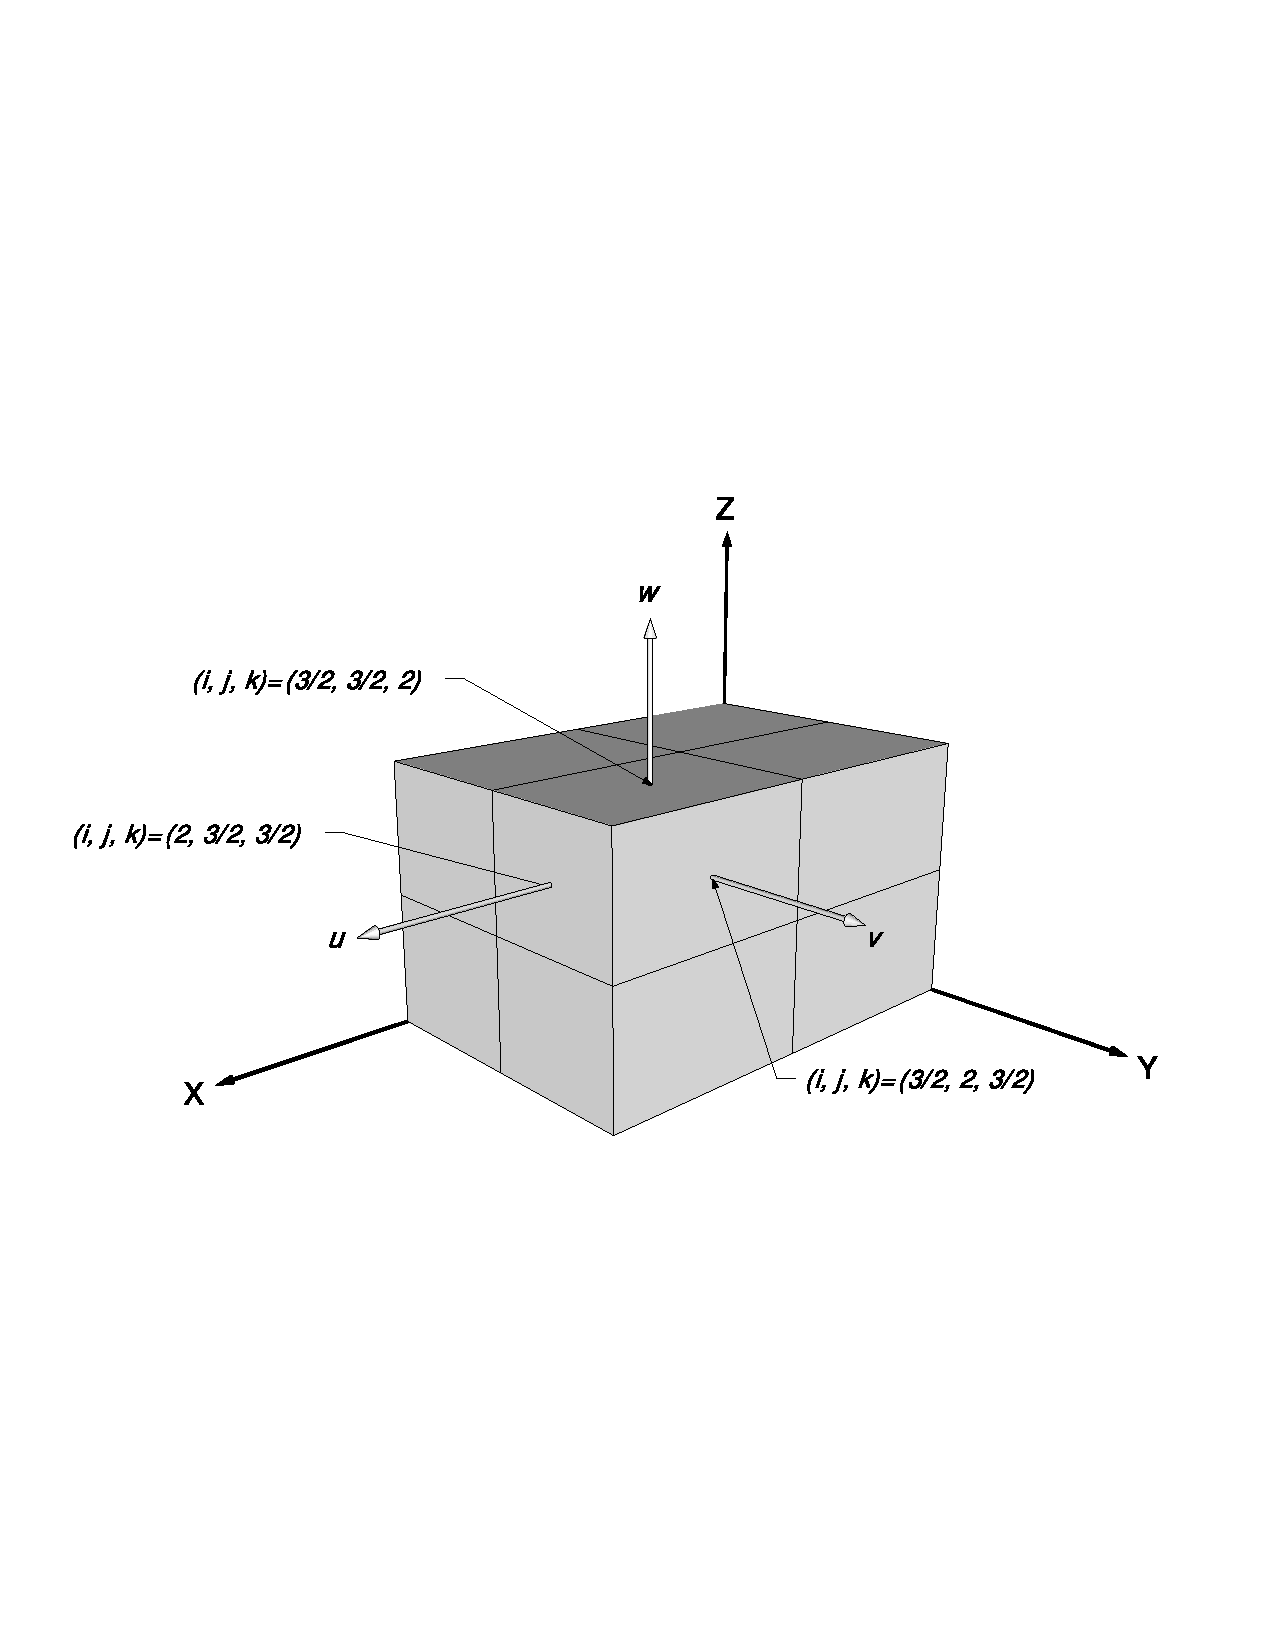
\includegraphics[width=5.6in]{../figures/Staggered/Staggered3D.pdf}
\label{fig:Staggered3D}
\caption{Staggered grid.}
\end{figure}

With the location of the value denoted by the subscript, Equation \ref{eqn:chap-FlowModel-momentum-u}, \ref{eqn:chap-FlowModel-momentum-v}, and \ref{eqn:chap-FlowModel-momentum-w} can be discretized as:
\begin {eqnarray}
u_{i+ \frac{1}{2},j,k}^{*} = u_{i+ \frac{1}{2},j,k}^{n}+ \Delta t
\{ -A(u_{i+ \frac{1}{2},j,k}^n)+E(u_{i+ \frac{1}{2},j,k}^n) \nonumber \\
-B(u_{i+
\frac{1}{2},j,k}^n)-g\frac{h_{i+1,j,k}^n-h_{i,j,k}^n}{\Delta x}
-\frac{1}{\rho}\frac{p_{d \ i+1,j,k}^n-p_{d \ i,j,k}^n}{ \Delta x}
\}
\end{eqnarray}
\begin {eqnarray}
v_{i,j+ \frac{1}{2},k}^{*} = v_{i,j+ \frac{1}{2},k}^{n}+ \Delta t
\{ -A(v_{i,j+ \frac{1}{2},k}^n)+E(v_{i,j+ \frac{1}{2},k}^n) \nonumber \\
-B(v_{i,j+
\frac{1}{2},k}^n)-g\frac{h_{i,j+1,k}^n-h_{i,j,k}^n}{\Delta y}
-\frac{1}{\rho}\frac{p_{d \ i,j+1,k}^n-p_{d \ i,j,k}^n}{ \Delta y}
\}
\end{eqnarray}
\begin {eqnarray}
w_{i,j,k+ \frac{1}{2}}^{*} = w_{i,j,k+ \frac{1}{2}}^{n}+ \Delta t
\{ -A(w_{i,j,k+ \frac{1}{2}}^n)+E(w_{i,j,k+ \frac{1}{2}}^n) \nonumber \\
-\frac{1}{\rho}\frac{p_{d \ i,j,k+1}^n-p_{d \ i,j,k}^n}{ \Delta z}
\}
\end{eqnarray}
The advection term is approximated by the central difference,
\begin{eqnarray}
A(u_{i+ \frac{1}{2} ,j,k})&=&( \frac{\partial uu}{\partial x} +  \frac{\partial
uv}{\partial y}+\frac{\partial uw}{\partial z})_{i+ \frac{1}{2} ,j, k}\nonumber\\
&=&\frac{(u^n_{i+1,j,k})^2-(u^n_{i,j,k})^2}{\Delta
x}+\frac{(uv)^n_{i+ \frac{1}{2} ,j+ \frac{1}{2} ,k}-(uv)^n_{i+
\frac{1}{2} ,j- \frac{1}{2} ,k}}{\Delta
y}\nonumber \\
& & + \frac{(uw)^n_{i+ \frac{1}{2} ,j,k + \frac{1}{2}} -(uw)^n_{i+
\frac{1}{2} ,j,k-1/2}}{\Delta z}
\end{eqnarray}
where the cell-centered velocity is approximated by the average of
neighboring points:
\begin{eqnarray*}
u^n_{i+1,j,k}&=&\frac{1}{2}(u^n_{i + \frac{3}{2},j,k}+u^n_{i+ \frac{1}{2} ,j,k})\\
u^n_{i,j,k}&=&\frac{1}{2}(u^n_{i+ \frac{1}{2} ,j,k}+u^n_{i-
\frac{1}{2} ,j,k})
\end{eqnarray*}
\begin{eqnarray*}
(uv)^n_{i+ \frac{1}{2} ,j+ \frac{1}{2} ,k}&=&\frac{1}{2}(u^n_{i+
\frac{1}{2} ,j,k}+u^n_{i+ \frac{1}{2} ,j+1,k})
\cdot \frac{1}{2}(v^n_{i,j+ \frac{1}{2} ,k}+v^n_{i+1,j+ \frac{1}{2} ,k})\\
(uv)^n_{i+ \frac{1}{2} ,j- \frac{1}{2} ,k}&=&\frac{1}{2}(u^n_{i+
\frac{1}{2} ,j,k}+u^n_{i+ \frac{1}{2} ,j-1,k}) \cdot
\frac{1}{2}(v^n_{i,j- \frac{1}{2} ,k}+v^n_{i+1,j- \frac{1}{2} ,k})
\end{eqnarray*}
\begin{eqnarray*}
(uw)^n_{i+ \frac{1}{2} ,j ,k+ \frac{1}{2}}&=&\frac{1}{2}(u^n_{i+
\frac{1}{2} ,j,k}+u^n_{i+ \frac{1}{2} ,j,k+1}) \cdot
\frac{1}{2}(w^n_{i,j ,k+ \frac{1}{2}}+w^n_{i+1,j ,k+
\frac{1}{2}})\\ (uw)^n_{i+ \frac{1}{2} ,j ,k-
\frac{1}{2}}&=&\frac{1}{2}(u^n_{i+ \frac{1}{2} ,j,k}+u^n_{i+
\frac{1}{2} ,j,k-1}) \cdot \frac{1}{2}(w^n_{i,j ,k-
\frac{1}{2}}+w^n_{i+1,j ,k- \frac{1}{2}})
\end{eqnarray*}
 The diffusion, barotropic, and baroclinic terms are:
\begin{eqnarray}
E(u_{i+ \frac{1}{2} ,j,k}) &=& \frac{\mu_h}{\Delta x^2} (u_{i +
\frac{3}{2},
j,k}-2u_{i+ \frac{1}{2} ,j,k} + u_{i- \frac{1}{2} , j,k})\nonumber \\
&+& \frac{\mu_h}{\Delta y^2} (u_{i + \frac{1}{2},
j+1,k}-2u_{i+ \frac{1}{2} ,j,k} + u_{i+ \frac{1}{2} ,j-1,k})\nonumber \\
&+& \frac{\mu_v}{\Delta z^2} (u_{i+ \frac{1}{2} ,j,k+1}-2u_{i+
\frac{1}{2} ,j,k}+u_{i+ \frac{1}{2} ,j,k-1})
\end{eqnarray}
\begin{equation}
B_{i+ \frac{1}{2} ,j,k}= \frac{g}{\Delta x \rho_o}
\sum_{\xi=k}^{nz_i}(\rho_{i+1,j,\xi} \ \Delta
z_{i+1,j,\xi}-\rho_{i,j,\xi} \ \Delta z_{i,j,\xi})
\end{equation}
 The free surface position at time step $n+1$ can be computed
from Equation \ref{continuity-surface}:
\begin{eqnarray}
h_{i,j}^{n+1}=h_{i,j}^n - \frac{\Delta t}{\Delta x}
\sum_{\xi=1}^{nz_{i,j}^n-1} ( \widetilde{u}_{i+ \frac{1}{2},j ,\xi}^{n +
\frac{1}{2}}  \cdot \Delta z_{i+ \frac{1}{2},j,\xi}^n -
\widetilde{u}_{i- \frac{1}{2},j,\xi}^{n + \frac{1}{2}}  \cdot
\Delta z_{i- \frac{1}{2},j , \xi}^n) \nonumber \\
- \frac{\Delta t}{\Delta y}
\sum_{\xi=1}^{nz_{i,j}^n-1} ( \widetilde{u}_{i,j+ \frac{1}{2},\xi}^{n +
\frac{1}{2}}  \cdot \Delta z_{i,j+ \frac{1}{2},\xi}^n -
\widetilde{u}_{i,j- \frac{1}{2},\xi}^{n + \frac{1}{2}}  \cdot
\Delta z_{i,j- \frac{1}{2}, \xi}^n)\nonumber \\
-\frac{1}{\Delta x}(  F_{i+ \frac{1}{2},j ,\ nz^n_{i,j}}- F_{i-
\frac{1}{2},j ,\ nz^n_{i,j}}+F_{i,j+ \frac{1}{2},\ nz^n_{i,j}}- F_{i,j-
\frac{1}{2},\ nz^n_{i,j}} )
\end{eqnarray}
where $nz^n_{i,j}$ is the surface cell at column $(i,j)$ at time $n$.
$\widetilde{u}$ is a weighted average of $u^n$ and $u^{n+1}$:
\begin{equation}
\widetilde{u}_{i+ \frac{1}{2},j,k}^{n + \frac{1}{2}}
=(1-\theta)u_{i+ \frac{1}{2},j,k}^{n}+\theta u_{i+ \frac{1}{2}
,j,k}^{n+1}
\end{equation}
$\Delta z_{i+ \frac{1}{2},j,k}^n$ is the average water depth of two
neighboring cells $(i,j,k)$ and $(i+ \frac{1}{2},j,k)$. The column is assumed to be filled from the bottom, so the average water depth of neighboring cells equals to $\Delta z$ except for the surface layer,
\begin{eqnarray*}
 &\textrm{if}\hspace{0.1in}&  k< nz_{i,j} \ \textrm{and} \ \ k< nz_{i+1,j} \nonumber \\
 &\hspace{0.4in}&\textrm{then} \hspace{0.3in} \Delta z_{i+ \frac{1}{2},j,k}=\Delta z \nonumber \\
 &\textrm{else}& \nonumber \\
 &\hspace{0.4in}& \Delta z_{i+ \frac{1}{2},j,k} =\f{h_{i,j}^n-(nz_{i,j}^n-1)\Delta z +h_{i+1,j}^n-(nz_{i+1,j}^n-1)\Delta z}{2}
\end{eqnarray*}
To prevent the over-emptying of the surface donor cell, the
out-flux at surface layer is limited to half of the water volume for two-dimensional case, or a quarter of the water volume for three-dimensional case,
\begin{equation}
\small
F_{i- \frac{1}{2} , j, \ nz^n_i}=\left\{
\begin{array}{ll}
\mathbf{Min}( \widetilde{u}_{i- \frac{1}{2},j,\ nz_i^n}^{\ n + \frac{1}{2}}
\Delta t\Delta z_{i- \frac{1}{2},j,\ nz_i^n}^n  \ , \ \frac{1}{4}
\Delta x \Delta y \Delta z_{i- \frac{1}{2},j,\ nz_i^n}^n \ )
\hspace{0.1in} \ \textrm{if} \ \widetilde{u}_{i- \frac{1}{2} ,j,\ nz_i^n}^{\ n
+ \frac{1}{2}} >0 \vspace{0.2in} \\
\widetilde{u}_{i- \frac{1}{2},j ,\ nz_i^n}^{\ n + \frac{1}{2}}  \Delta t\Delta z_{i- \frac{1}{2},j,\ nz_i^n}^n \hspace{0.1in} \textrm{if} \ \widetilde{u}_{i- \frac{1}{2},j,\ nz_i^n}^{\ n + \frac{1}{2}} <0 \\
\end{array}\right.
\end{equation}
\begin{equation}
\small
F_{i+ \frac{1}{2},j, \ nz^n_i}=\left\{
\begin{array}{ll}
\mathbf{Max} ( \widetilde{u}_{i+ \frac{1}{2},j,\ nz_i^n}^{\ n +
\frac{1}{2}}  \Delta t\Delta z_{i+ \frac{1}{2},j,\ nz_i^n}^n \ , \
-\frac{1}{4} \Delta x \Delta y \Delta z_{i+ \frac{1}{2},j,\
nz_i^n}^n \ ) \hspace{0.1in} \ \textrm{if} \ \widetilde{u}_{i+ \frac{1}{2},j,\ nz_i^n}^{\ n + \frac{1}{2}} <0 \vspace{0.2in} \\
\widetilde{u}_{i+ \frac{1}{2},j,\ nz_i^n}^{\ n + \frac{1}{2}}  \Delta t \Delta z_{i+ \frac{1}{2},j,\ nz_i^n}^n \hspace{0.1in} \textrm{if} \ \widetilde{u}_{i+ \frac{1}{2},j,\ nz_i^n}^{\ n + \frac{1}{2}} >0 \\
\end{array}\right.
\end{equation}
To simplify the free surface model, the surface level can be assumed to have small variations from the top layer, therefore the free surface position is approximated as:
\begin{eqnarray}
h_{i,j}^{n+1}=h_{i,j}^n - \frac{\Delta t}{\Delta x}
\sum_{\xi=1}^{nz} ( u_{i+ \frac{1}{2},j ,\xi}^{n +
\frac{1}{2}}  \cdot \Delta z_{i+ \frac{1}{2},j,\xi}^n -
\widetilde{u}_{i- \frac{1}{2},j,\xi}^{n + \frac{1}{2}}  \cdot
\Delta z_{i- \frac{1}{2},j , \xi}^n) \nonumber \\
- \frac{\Delta t}{\Delta y}
\sum_{\xi=1}^{nz} ( u_{i,j+ \frac{1}{2},\xi}^{n +
\frac{1}{2}}  \cdot \Delta z_{i,j+ \frac{1}{2},\xi}^n -
u_{i,j- \frac{1}{2},\xi}^{n + \frac{1}{2}}  \cdot
\Delta z_{i,j- \frac{1}{2}, \xi}^n)
\end{eqnarray}
To prevent the instability caused by steep waves, the free surface position can be averaged by that of neighboring nodes in two dimensional case\cite{Turnbull2003}:
\begin{equation}
h_i^*=\frac{1}{16}(-h_{i-2}+4h_{i-1}+10h_{i}+4h_{i+1}-h_{i+2})
\end{equation}
The kinematic boundary condition may be used to specify the vertical
velocity near the surface,
\begin{equation}
w_{i,j,\ nz_{i,j}^n + \frac{1}{2}} ^{n+1} = (h_{i,j}^{n+1}-h_{i,j}^{n})/ \Delta
t
\end{equation}
In the simplified free surface model the surface vertical velocity can be computed from the continuity equation,
\ba
\small
w_{i,j,\ nz + \frac{1}{2}} = w_{i,j,\ nz - \frac{1}{2}}
-(u_{i+\frac{1}{2},j, nz}-u_{i-\frac{1}{2},j, nz} )\Delta z/\Delta x \nonumber \\
-(v_{i,j+\frac{1}{2}, nz}-v_{i,j-\frac{1}{2}, nz} )\Delta z/\Delta y
\ea

